\documentclass[14pt]{beamer} %Makes presentation
%\documentclass[handout]{beamer} %Makes Handouts
\usetheme{Singapore} %Gray with fade at top
\useoutertheme[subsection=false]{miniframes} %Supppress subsection in header
\useinnertheme{rectangles} %Itemize/Enumerate boxes
\usecolortheme{seagull} %Color theme
\usecolortheme{rose} %Inner color theme

\definecolor{light-gray}{gray}{0.75}
\definecolor{dark-gray}{gray}{0.55}
\setbeamercolor{item}{fg=light-gray}
\setbeamercolor{enumerate item}{fg=dark-gray}

\setbeamertemplate{navigation symbols}{}
%\setbeamertemplate{mini frames}[default]
\setbeamercovered{dynamics}
\setbeamerfont*{title}{size=\Large,series=\bfseries}

%\setbeameroption{notes on second screen} %Dual-Screen Notes
%\setbeameroption{show only notes} %Notes Output

\setbeamertemplate{frametitle}{\vspace{.5em}\bfseries\insertframetitle}
\newcommand{\heading}[1]{\noindent \textbf{#1}\\ \vspace{1em}}

\usepackage{bbding,color,multirow,times,ccaption,tabularx,graphicx,verbatim,booktabs,fixltx2e}
\usepackage{colortbl} %Table overlays
\usepackage[english]{babel}
\usepackage[latin1]{inputenc}
\usepackage[T1]{fontenc}
\usepackage{lmodern}

%\author[]{Thomas J. Leeper}
\institute[]{
  \inst{}%
  Department of Political Science and Government\\Aarhus University
}

\usepackage{tikz}
\usetikzlibrary{shapes,arrows}
\usetikzlibrary{decorations.pathreplacing}

\title{Research Designs for Causal Inference}

\date[]{March 10, 2015}

\begin{document}

\frame{\titlepage}

\frame{\tableofcontents}

\section{Background}

\frame{
	\frametitle{Background}
	\begin{itemize}\itemsep1.5em
		\item The experimental ideal!
		\item All observational studies require an \textbf{identification strategy}
		\item We've been focusing on conditioning (via matching and/or regression)
		\item Today's lecture is about quasi-experimental designs
	\end{itemize}
}

\frame{
	\frametitle{What is a Quasi-Experiment?}
	\begin{itemize}\itemsep1em
		\item<1-> A situation where a real-world event induces an exogenous change (or ``shock'') in an independent variable
		\item<2-> Also sometimes called \textit{``natural'' experiments}
		\item<3-> Can anyone think of examples?
	\end{itemize}
}

\frame{
	\frametitle{Design Trumps Analysis}
	\begin{itemize}\itemsep2em
		\item Observational studies are hard because we need to have a convincing causal theory and have observed all causally relevant variables
		\item Quasi-Experiments potentially save us from needing a complete and fully observed set of causal variables
		\item In a quasi-experiment, we can treat our data (almost) as-if they are from an experiment
	\end{itemize}
}

\section[IV]{Instrumental Variables}
\frame{\tableofcontents[currentsection]}

\frame{
	\frametitle{A little history}
	\begin{itemize}\itemsep1em
		\item Have been used for a very long time (since Wright 1928)
		\item Very popular identification strategy in economics
		\item Just starting to become widespread in political science
	\end{itemize}
}

\frame{
	\frametitle{When would we use IV?}
	\begin{itemize}\itemsep1em
		\item We are interested in the effect of $X \rightarrow Y$
		\item This relationship is confounded by unobservables
		\item We cannot manipulate $X$ (i.e., no experiments)
		\item How can we identify the effect $X \rightarrow Y$?
	\end{itemize}
}

\frame{
	\begin{center}
		\begin{tikzpicture}[>=latex',circ/.style={draw, shape=circle, node distance=5cm, line width=1.5pt}]
		\draw[->] (0,0) node[left] (X) {X} -- (5,0) node[right] (Y) {Y};
		\draw[->] (-3,4) node[above] (Z) {Z} -- (X);
		\draw[->] (Z) -- (Y);
		\draw[->] (5,2) node[above] (A) {A} -- (Y);
		\draw<1>[->] (-2,0) node[left] (B) {B} -- (X);
		\draw<2>[->,red,thick] (-2,0) node[left] (B) {\color{red}{B}} -- (X);
		\draw[->] (X) -- (2,-2) node[right] (C) {C};
		\end{tikzpicture}
	\end{center}
}

\frame{
	\frametitle{What is ``instrumental''?}
	\begin{enumerate}\itemsep1em
		\item \alert<2>{serving as a crucial means, agent, or tool}
		\item of, relating to, or done with an instrument or tool
		\item relating to, composed for, or performed on a musical instrument
		\item of, relating to, or being a grammatical case or form expressing means or agency
	\end{enumerate}
}

\frame{
	\frametitle{What is ``instrumental''?}
	\begin{itemize}\itemsep2em
		\item $B$ must be a crucial cause of $X$'s effect on $Y$
		\item $B$ is the quasi-experimental shock to the causal process in our graph
	\end{itemize}	
}

\frame{
	\frametitle{Formal Definition}
	An \textbf{instrumental variable} is a variable that satisfies two properties:\\
	\begin{enumerate}\itemsep1em
		\item Exogeneity\\ % Not testable
			\begin{itemize}
				\item $B$ temporally precedes $X$
				\item $Cov(B, \epsilon) = 0$
			\end{itemize}
		\item Relevance\\ % Is testable
			\begin{itemize}
				\item $B$ causes $X$
				\item $Cov(B, X) \neq 0$
			\end{itemize}
	\end{enumerate}
}

\frame{
	\frametitle{Example: Returns to Schooling}
	\begin{center}
		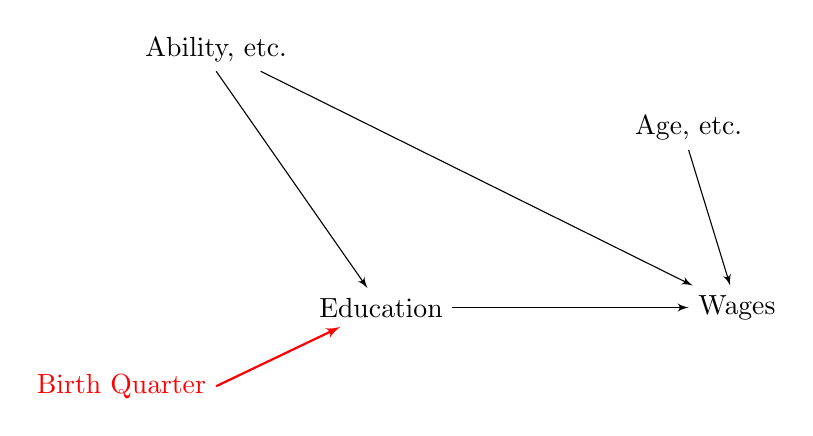
\begin{tikzpicture}[>=latex',circ/.style={draw, shape=circle, node distance=5cm, line width=1.5pt}]
		\draw[->] (0,0) node[left] (X) {Education} -- (3,0) node[right] (Y) {Wages};
		\draw[->] (-3,3) node[above] (Z) {Ability, etc.} -- (X);
		\draw[->] (Z) -- (Y);
		\draw[->] (3,2) node[above] (A) {Age, etc.} -- (Y);
		\draw<2>[->,red,thick] (-3,-1) node[left] (B) {\color{red}{Birth Quarter}} -- (X);
		\end{tikzpicture}
	\end{center}
}

\frame{
	\frametitle{How IV Works I}
	\begin{itemize}\itemsep1em
		\item Start with case where $B$ is a 0,1 indicator
		\item To identify the effect $X \rightarrow Y$, all we need is $B$
		\item We don't need to worry about other omitted variables, because the as-if-random instrument is doing all the heavy lifting for us
		\item But we don't learn anything about the rest of the causal graph
	\end{itemize}
}

\frame{
	\frametitle{How IV Works II (Wald)}
	\begin{itemize}\itemsep1em
		\item Imagine two effects:
		\begin{align}
		ITT_y & = E[y_i | b_i = 1] - E[y_i | b_i = 0]\\
		ITT_x & = E[x_i | b_i = 1] - E[x_i | b_i = 0]
		\end{align}
		\item IV estimates the LATE: $\dfrac{ITT_y}{ITT_x}$
		\item In a regression, this is:\\
			$E[y_i|b_i] = \beta_0 + \text{LATE} \times E[x_i|b_i]$
	\end{itemize}
}

\begin{frame}[fragile]
	\frametitle{How IV Works III (2SLS)}
	\begin{itemize}\itemsep1em
		\item Regress $x$ on $b$:\\
			$\hat{x}_i = \hat{\gamma}_0 + \hat{\gamma}_1 b_i + g_i$
		\item Regression $y$ on $\hat{x}$:\\
			$\hat{y}_i = \hat{\beta}_0 + \hat{\beta}_1 \hat{x}_i + e_i$
		\item Both $x$ and $b$ can be continuous
		\item We can also have multiple $b$'s and multiple $x$'s
		\item In Stata:\\
			\small
			\begin{verbatim}
			ivregress 2sls Y covariates (X = B), first
			\end{verbatim}
	\end{itemize}
\end{frame}

\frame{
	\frametitle{Standard Errors in IV}
	\begin{itemize}\itemsep2em
	\item SEs are larger in IV than OLS
	\item Second-stage can use ``robust'' SEs to account for heteroskedasticity
	\item The weaker the instrument, the larger the SEs
	\end{itemize}
}

\frame{
	\frametitle{IV Diagnostics}
	\begin{itemize}\itemsep2em
	\item Assess relevance of instrument
		\begin{itemize}
		\item Examine first-stage equation
		\item \texttt{estat firststage}
		\end{itemize}
	\item<2-> Durbin-Wu-Hausman Test (exclusion restriction)\\
		\begin{itemize}
		\item Do residuals from the first stage relate to $y$?
		\item $y = \beta_0 + \beta_1 x_{\text{Confounded}} + \beta_2 \hat{\eta} + e$
		\item $\eta$ are the residuals from the first stage
		\item In Stata: \texttt{estat endogenous}
		\end{itemize}
	\end{itemize}
}

\frame{
	\frametitle{IV Diagnostics}
	\begin{itemize}\itemsep1em
	\item Depending on number of confounded variables and number of instruments, model is:
		\begin{itemize}
		\item Exactly identified
		\item Overidentified
		\item Underidentified
		\end{itemize}
	\item Test of overidentified models:
		\begin{itemize}
		\item Evaluate null hyp. that all instruments are relevant
		\item Rejection means at least one instrument irrelevant
		\item In Stata: \texttt{estat overid}
		\end{itemize}
	\item Not applicable in most real-world situations
	\end{itemize}
}


\frame{
	\frametitle{SATE vs. LATE}
	\begin{itemize}\itemsep1em
	\item IV estimate \textit{local} to the variation in $X$ that is due to variation $B$ (i.e., the LATE)
	\item This matters if effects are \textit{heterogeneous}
	\item LATE is effect for those who \textit{comply} with instrument
	\item Four subpopulations:
		\begin{itemize}
		\item Compliers: $X = 1$ only if $B = 1$
		\item Always-takers: $X = 1$ regardless of $B$
		\item Never-takers: $X = 0$ regardless of $B$
		\item Defiers: $X = 1$ only if $B = 0$
		\end{itemize}
	\end{itemize}
}
% - Compliers: military service if drafted
% - Always-takers: military service regardless of draft
% - Never-takers: no military service regardless of draft (maybe medically ineligible)
% - Defiers: military service only if not drafted

% ITT_y
% 1. For Always-takers and Never-takers, the effect is zero because we see the same potential outcomes for them regardless of the value of Z. Z does not affect X for these individuals, so their ITT is 0.
% 2. We assume no defiers.
% 3. What is left is the ITT for compliers (the effect of the instrument on Y) times Pr(Complier). But we want to know the effect of X on Y for these individuals. To do that we need to know how many compliers there are in order to divide out to get just the ATE for compliers.

\frame{
	\frametitle{SATE vs. LATE}
	\begin{align*}
    SATE = & \pi_{Compliers} * ITT_{Compliers}\\
	     & + \only<1-2>{\pi_{Always-Takers} * ITT_{Always-Takers}}\only<3->{0}\\
	     & + \only<1-2>{\pi_{Never-Takers} * ITT_{Never-Takers}}\only<3->{0}\\
	     & + \only<1-4>{\pi_{Defiers} * ITT_{Defiers}}\only<5->{0}
	\end{align*}
	\begin{itemize}
	\item We don't know which subpopulation each unit is from
	\item<2-> Effect for always- and never-takers is zero
	\item<4-> Assume no defiers (monotonicity)
	\end{itemize}
}


\frame{
	\frametitle{SATE vs. LATE}
	\begin{align*}
	LATE & = \dfrac{SATE}{\pi_{Complier}} \onslide<2->{= \dfrac{E[Y|B=1] - E[Y|B=0]}{\pi_{Complier}}}\\[1em]
	\only<3>{\pi_{Complier} & = Pr(X=1|B=1) - Pr(X=1|B=0)\\}
	\onslide<4->{& = \dfrac{ITT_y}{ITT_x}}
	\end{align*}
	\begin{itemize} %\itemsep1em
	\item<5-> Sometimes also called CATE or CACE
	\item<6-> Is this what we want to know?
	\end{itemize}
}
%  1. For Always-takers and Never-takers, the effect is zero because we see the same potential outcomes for them regardless of the value of Z. Z does not affect X for these individuals, so their ITT is 0.
% 2. We assume no defiers.
% 3. What is left is the ITT for compliers (the effect of the instrument on Y) times Pr(Complier). But we want to know the effect of X on Y for these individuals. To do that we need to know how many compliers there are in order to divide out to get just the ATE for compliers.

% $\pi_{Compliers}$
% Left-hand is Pr(Always-takers) + Pr(Compliers). There are no Never-takers by definition.
% Right-hand is Pr(Never-takers) + Pr(Compliers). There are no Always-takers by definition.


\frame{
	\frametitle{Finding Instruments}
	\begin{itemize}\itemsep1em
		\item Forward, not backward, causal inference
		\item Most instruments are not things we care about
			\begin{itemize}
				\item Weather, disasters
				\item Geography, climate
				\item Lotteries
			\end{itemize}
		\item A good instrument is one that satisfies both of our conditions, so we need:
			\begin{itemize}
				\item A good story about exogeneity
				\item Evidence that instrument is \textit{strong}
			\end{itemize}
	\end{itemize}
}

\frame{
	\frametitle{Instrumental Variables Activity}
	\begin{itemize}\itemsep2em
		\item Read each scenario
		\item Assess \textbf{exogeneity} and \textbf{relevance}
		\item Discuss with the person sitting next to you
	\end{itemize}
}

\frame{\frametitle{Questions about IV?}}




\section[RDD]{Regression Discontinuity Designs}
\frame{\tableofcontents[currentsection]}

\frame{
	\frametitle{Example: Maimonides' Rule}
	\begin{enumerate}\itemsep2em
		\item<2-> What is Maimonides' Rule?
		\item<3-> Why is it a valid (credible) instrument? (Or why isn't it?)
		\item<4-> How does it differ from a randomized experiment?
	\end{enumerate}
}

\frame{
	\begin{center}
		\begin{tikzpicture}[>=latex',circ/.style={draw, shape=circle, node distance=5cm, line width=1.5pt}]
		\draw[->] (0,0) node[left] (X) {Class Size} -- (3,0) node[right] (Y) {Test Scores};
		\draw[->] (-2,3) node[above] (Z) {Z} -- (X);
		\draw[->] (Z) -- (Y);
		\draw[->,red,thick] (-2,-2) node[left] (B) {\color{red}{Grade Size}} -- (X);
		\end{tikzpicture}
	\end{center}
}



\frame{
	\frametitle{How RDD Works}
	\begin{enumerate}\itemsep1em
	\item Find a consequential threshold
		\begin{itemize}
		\item Examples?
		\end{itemize}
	\item Causal inference is about comparisons
		\begin{itemize}
		\item In an experiment, $X$ is randomly assigned
		\item In matching or regression, we compare units that differ only in $X$ but are similar in $Z$
		\end{itemize}
	\item In RDD, $X$ is not randomly assigned and there is no \textit{covariate overlap}
		\begin{itemize}
		\item $B$ causally determines $X$, so units with different values of $X$ also differ in their value of $B$
		\item compare units that are as similar as possible
		\end{itemize}
	\end{enumerate}
}

% graphs showing changes in slope versus changes in level

\frame{
	\frametitle{Regression Discontinuity}
	\begin{center}
	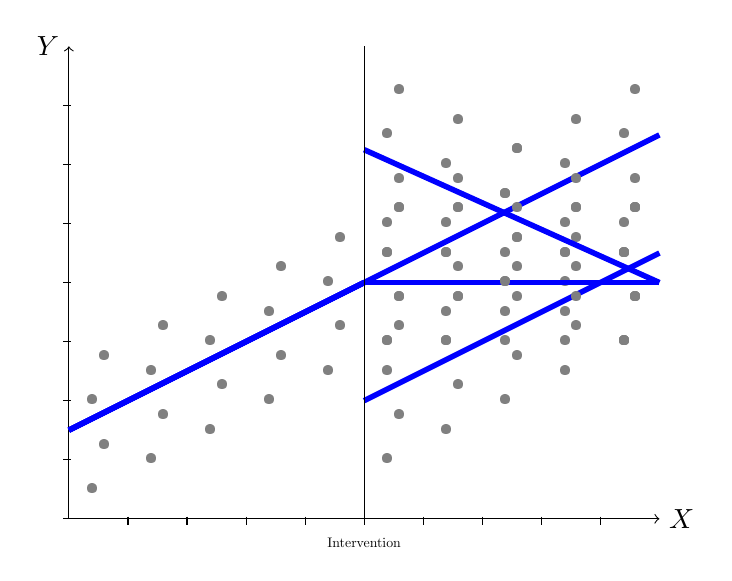
\begin{tikzpicture}[scale=0.75]
 	\draw[->] (0,0) -- (10,0) node[right] (xaxis) {$X$};
	\draw[->] (0,0) -- (0,8) node[left] (yaxis) {$Y$};
	% x ticks
	\foreach \x in {1,2,...,9}
      	\draw (\x,1pt) -- (\x,-3pt) node[anchor=north] {};
	% y ticks
	\foreach \y in {0,...,7}
       \draw (1pt,\y) -- (-3pt,\y) node[anchor=east] {};
	
	\foreach \Point in
      {(0.4,0.50), (0.6,1.25), (0.4,2.00), (0.6,2.75),
       (1.4,1.00), (1.6,1.75), (1.4,2.50), (1.6,3.25),
       (2.4,1.50), (2.6,2.25), (2.4,3.00), (2.6,3.75),
       (3.4,2.00), (3.6,2.75), (3.4,3.50), (3.6,4.25),
       (4.4,2.50), (4.6,3.25), (4.4,4.00), (4.6,4.75)}{
        \node<2->[gray] at \Point {\textbullet};
     };
	\foreach \Point in
       {(5.4,3.00), (5.6,3.75), (5.4,4.50), (5.6,5.25),
       (6.4,3.50), (6.6,4.25), (6.4,5.00), (6.6,5.75),
       (7.4,4.00), (7.6,4.75), (7.4,5.50), (7.6,6.25),
       (8.4,4.50), (8.6,5.25), (8.4,6.00), (8.6,6.75),
       (9.4,5.00), (9.6,5.75), (9.4,6.50), (9.6,7.25)}{
        \node<2-4>[gray] at \Point {\textbullet};
     };
	\draw<3-4>[blue,line width=2pt] (0.00,1.5) -- (10.00,6.50);

	\foreach \Point in
       {(5.4,1.00), (5.6,1.75), (5.4,2.50), (5.6,3.25),
       (6.4,1.50), (6.6,2.25), (6.4,3.00), (6.6,3.75),
       (7.4,2.00), (7.6,2.75), (7.4,3.50), (7.6,4.25),
       (8.4,2.50), (8.6,3.25), (8.4,4.00), (8.6,4.75),
       (9.4,3.00), (9.6,3.75), (9.4,4.50), (9.6,5.25)}{
        \node<5-6>[gray] at \Point {\textbullet};
     };
	\draw<6>[blue,line width=2pt] (0.00,1.5) -- (5.00,4.00);
	\draw<6>[blue,line width=2pt] (5.00,2.00) -- (10.00,4.50);
			  
	\foreach \Point in
       {(5.4,3.00), (5.6,3.75), (5.4,4.50), (5.6,5.25),
       (6.4,3.00), (6.6,3.75), (6.4,4.50), (6.6,5.25),
       (7.4,3.00), (7.6,3.75), (7.4,4.50), (7.6,5.25),
       (8.4,3.00), (8.6,3.75), (8.4,4.50), (8.6,5.25),
       (9.4,3.00), (9.6,3.75), (9.4,4.50), (9.6,5.25)}{
        \node<7-8>[gray] at \Point {\textbullet};
     };
	\draw<8>[blue,line width=2pt] (0.00,1.5) -- (5.00,4.00);
	\draw<8>[blue,line width=2pt] (5.00,4.00) -- (10.00,4.00);
			  
	\foreach \Point in
       {(5.4,5.00), (5.6,5.75), (5.4,6.50), (5.6,7.25),
       (6.4,4.50), (6.6,5.25), (6.4,6.00), (6.6,6.75),
       (7.4,4.00), (7.6,4.75), (7.4,5.50), (7.6,6.25),
       (8.4,3.50), (8.6,4.25), (8.4,5.00), (8.6,5.75),
       (9.4,3.00), (9.6,3.75), (9.4,4.50), (9.6,5.25)}{
        \node<9-10>[gray] at \Point {\textbullet};
     };
	\draw<10>[blue,line width=2pt] (0.00,1.5) -- (5.00,4.00);
	\draw<10>[blue,line width=2pt] (5.00,6.25) -- (10.00,4.00);
			  
	% intervention
	\draw<4-> (5,-0.25) node[below, scale=0.5] (IV) {Intervention};
	\draw<4-> (5,0) -- (5,8);	
	
	\end{tikzpicture}
	\end{center}
}

\frame{
	\frametitle{Is There A Discontinuity?}
	\begin{center}
	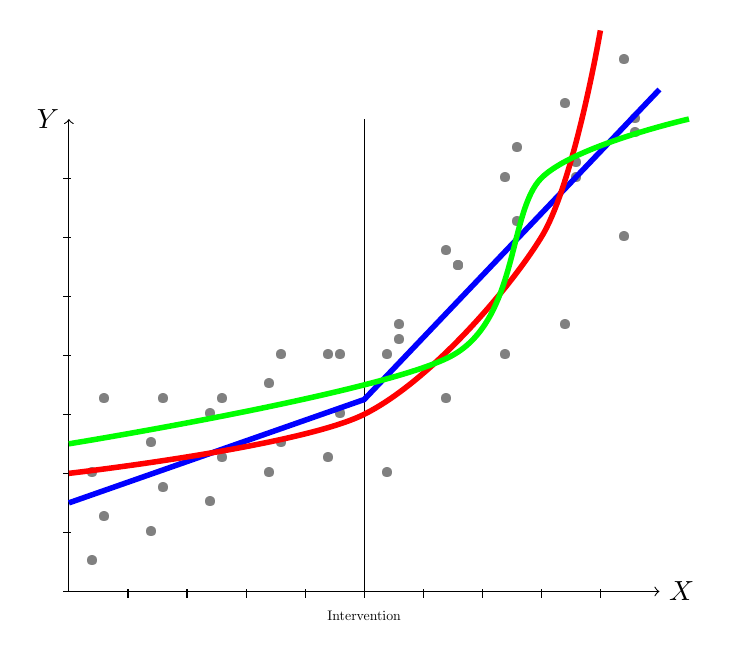
\begin{tikzpicture}[scale=0.75]
 	\draw[->] (0,0) -- (10,0) node[right] (xaxis) {$X$};
	\draw[->] (0,0) -- (0,8) node[left] (yaxis) {$Y$};
	% x ticks
	\foreach \x in {1,2,...,9}
      	\draw (\x,1pt) -- (\x,-3pt) node[anchor=north] {};
	% y ticks
	\foreach \y in {0,...,7}
       \draw (1pt,\y) -- (-3pt,\y) node[anchor=east] {};
	
	\foreach \Point in
      {(0.4,0.50), (0.6,1.25), (0.4,2.00), (0.6,3.25),
       (1.4,1.00), (1.6,1.75), (1.4,2.50), (1.6,3.25),
       (2.4,1.50), (2.6,2.25), (2.4,3.00), (2.6,3.25),
       (3.4,2.00), (3.6,2.50), (3.4,3.50), (3.6,4.0),
       (4.4,2.25), (4.6,3.00), (4.4,4.00), (4.6,4.00)}{
        \node<2->[gray] at \Point {\textbullet};
     };
	\foreach \Point in
       {(5.4,2.00), (5.6,4.25), (5.4,4.00), (5.6,4.5),
       (6.4,3.25), (6.6,5.50), (6.4,5.75), (6.6,5.50),
       (7.4,4.00), (7.6,6.25), (7.4,7.00), (7.6,7.50),
       (8.4,4.50), (8.6,7.0), (8.4,8.25), (8.6,7.25),
       (9.4,6.00), (9.6,7.75), (9.4,9.00), (9.6,8.00)}{
        \node<2->[gray] at \Point {\textbullet};
     };

	% intervention
	\draw<3-> (5,-0.25) node[below, scale=0.5] (IV) {Intervention};
	\draw<3-> (5,0) -- (5,8);	
	\draw<4->[blue,line width=2pt] (0.00,1.5) -- (5.00,3.25) -- (10.00,8.50);
	\draw<5->[red,line width=2pt] plot [smooth] coordinates {(0,2) (5,3) (8,6) (9,9.5)};
	\draw<6>[green,line width=2pt] plot [smooth] coordinates {(0,2.5) (6.5,4) (8,7) (10.5,8)};
	
	\end{tikzpicture}
	\end{center}
}



\frame{
	\frametitle{``Sharp'' and ``Fuzzy'' RDD}
	\begin{itemize}\itemsep1em
		\item If a threshold perfectly causes $X$, then it produces a \textbf{sharp} discontinuity
			\begin{itemize}
			\item Potentially analyze as an experiment
			\end{itemize}
		\item<2-> If a threshold imperfectly (probabilistically) causes $X$, then it produces a \textbf{fuzzy} discontinuity
			\begin{itemize}
			\item<3-> Analyze using Instrumental Variables
			\begin{equation*}
			  B=\begin{cases}
			    1, & \text{if $x > \text{threshold}$}\\
			    0, & \text{if $x < \text{threshold}$}
			  \end{cases}
			\end{equation*}
			\item<3-> Need to choose bandwidths
			\end{itemize}
	\end{itemize}
}


\frame{
	\frametitle{Sharp vs. Fuzzy RDD}
	\begin{center}
	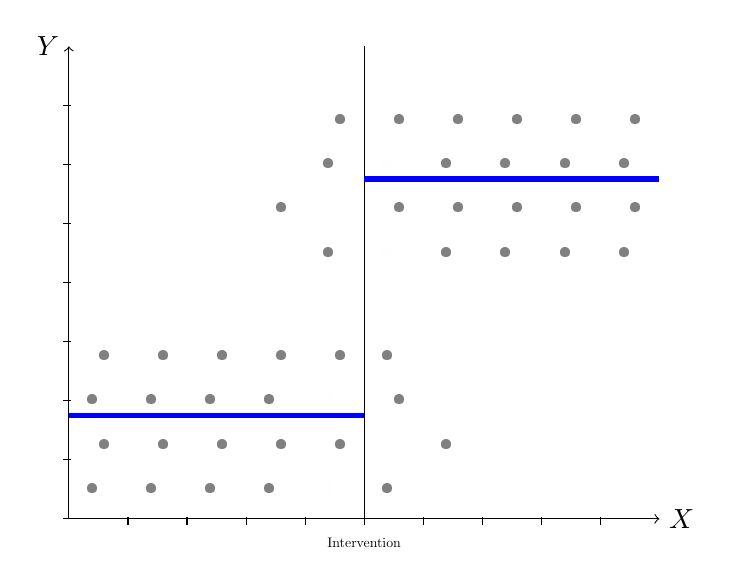
\begin{tikzpicture}[scale=0.75]
 	\draw[->] (0,0) -- (10,0) node[right] (xaxis) {$X$};
	\draw[->] (0,0) -- (0,8) node[left] (yaxis) {$Y$};
	% x ticks
	\foreach \x in {1,2,...,9}
      	\draw (\x,1pt) -- (\x,-3pt) node[anchor=north] {};
	% y ticks
	\foreach \y in {0,...,7}
       \draw (1pt,\y) -- (-3pt,\y) node[anchor=east] {};
	% intervention
	\draw (5,-0.25) node[below, scale=0.5] (IV) {Intervention};
	\draw (5,0) -- (5,8);	
	
	\foreach \Point in
      {(0.4,0.50), (0.6,1.25), (0.4,2.00), (0.6,2.75),
       (1.4,0.50), (1.6,1.25), (1.4,2.00), (1.6,2.75),
       (2.4,0.50), (2.6,1.25), (2.4,2.00), (2.6,2.75),
       (3.4,0.50), (3.6,1.25), (3.4,2.00), (3.6,2.75),
       (4.4,0.50), (4.6,1.25), (4.4,2.00), (4.6,2.75)}{
        \node [gray] at \Point {\textbullet};
     };
	\foreach \Point in
      {(5.4,4.50), (5.6,5.25), (5.4,6.00), (5.6,6.75),
       (6.4,4.50), (6.6,5.25), (6.4,6.00), (6.6,6.75),
       (7.4,4.50), (7.6,5.25), (7.4,6.00), (7.6,6.75),
       (8.4,4.50), (8.6,5.25), (8.4,6.00), (8.6,6.75),
       (9.4,4.50), (9.6,5.25), (9.4,6.00), (9.6,6.75)}{
        \node [gray] at \Point {\textbullet};
     };
	\draw [blue,line width=2pt] (0.00,1.75) -- (5.00,1.75);
	\draw [blue,line width=2pt] (5.00,5.75) -- (10.00,5.75);
	\foreach \Point in
	   {(5.4,0.50), (6.4,1.25), (5.6,2.00), (5.4,2.75),
	    (4.4,4.50), (3.6,5.25), (4.4,6.00), (4.6,6.75)}{
    	 \node<2-> [gray] at \Point {\textbullet};
	  };
	\foreach \Point in
	   {(5.4,4.50), (5.4,6.00), (4.4,0.50), (4.4,2.00)}{
    	 \node<2-> [white] at \Point {\large \textbullet};
	  };
	\end{tikzpicture}
	\end{center}
}



% modelling RDD

\frame{
	\frametitle{Modelling Fuzzy RDD}
}




\frame{
	\frametitle{Problems with Discontinuities}
	\begin{itemize}\itemsep1em
		\item Discontinuities are exploitable
		\item Campbell's Law:\\
		\textit{The more any quantitative social indicator (or even some qualitative indicator) is used for social decision-making, the more subject it will be to corruption pressures and the more apt it will be to distort and corrupt the social processes it is intended to monitor.}
		\item Compensatory rivalry and equalization
	\end{itemize}
}

\frame{\frametitle{Questions about RDD?}}



\section[ITS]{Interrupted Time-Series}
\frame{\tableofcontents[currentsection]}


\frame<1>[label=itshow]{
	\frametitle{How ITS Works}
	\begin{itemize}\itemsep0.5em
		\item Identify an exogenous shock in $X$ that might affect $Y$
		\item Look at $Y$ before ($t$) and after ($t+1$) the shock
		\item We only observe one manifest outcome at each point in time
		\item<2-> To make a causal inference, we need:
			\begin{itemize}
				\item $Y_{0,t}$ and $Y_{1,t}$, or
				\item $Y_{0,t+1}$ and $Y_{1,t+1}$
			\end{itemize}
		\item<2-> Use pre-post comparisons to infer the value of unobserved potential outcomes		
	\end{itemize}
}

\frame<1-2>[label=its]{
	\begin{center}
	\begin{tikzpicture}[scale=0.7]
    \draw[->] (0,0) -- (11,0) node[right] (xaxis) {\small time};
    \draw[->] (0,0) -- (0,11) node[left] (yaxis) {};
    % x ticks
    \foreach \x in {1,2,...,10}
       	\draw (\x,1pt) -- (\x,-3pt) node[anchor=north] {};
    % y ticks
    \foreach \y in {0,...,10}
         \draw (1pt,\y) -- (-3pt,\y) node[anchor=east] {};
    % intervention
    \draw (5.5,-0.25) node[below, scale=0.5] (IV) {Intervention};
    \draw (5.5,0) -- (5.5,11);

	\draw<1>[thick,blue] (5,10) -- (6,7);
	\draw<2->[dashed,thick,blue] (5,10) -- (6,7);
	\draw<2->[thick,blue] (1,4) -- (2,2) -- (3,5) -- (4,3) -- (5,10);
	\draw<2->[thick,blue] (6,7) -- (7,6) -- (8,6) -- (9,4) -- (10,3);
	
	\draw<3->[thick,red] (1,8) -- (2,8.5) -- (3,7.5) -- (4,8.5) -- (5,8) -- (6,7.5) -- (7,8.5) -- (8,8) -- (9,8.5) -- (10,7.5);
	\end{tikzpicture}
	\end{center}
}

\againframe<1-2>{itshow}


\frame{
	\begin{center}
	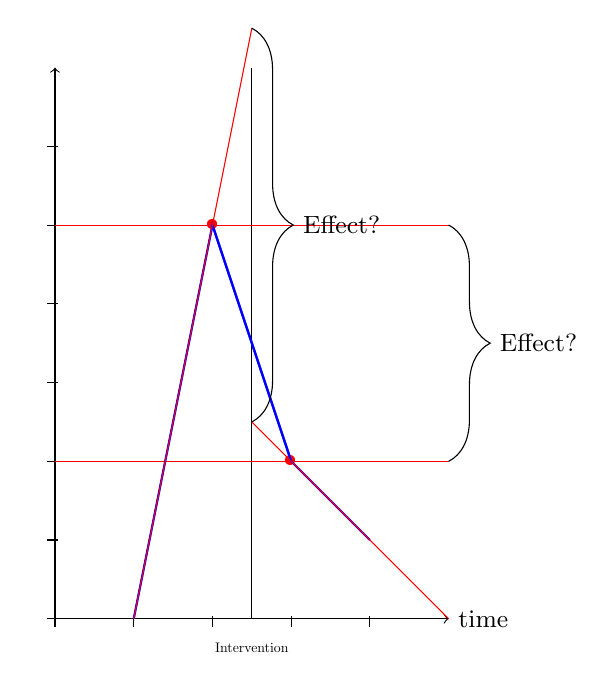
\begin{tikzpicture}[scale=1]
    \draw[->] (0,0) -- (5,0) node[right] (xaxis) {\small time};
    \draw[->] (0,0) -- (0,7) node[left] (yaxis) {};
    % x ticks
    \foreach \x in {0,...,4}
       	\draw (\x,1pt) -- (\x,-3pt) node[anchor=north] {};
    % y ticks
    \foreach \y in {0,...,6}
         \draw (1pt,\y) -- (-3pt,\y) node[anchor=east] {};
    % intervention
    \draw (2.5,-0.25) node[below, scale=0.5] (IV) {Intervention};
    \draw (2.5,0) -- (2.5,7);

	\draw[thick,blue] (2,5) -- (3,2);
	\node<2-> [red] at (2,5) {\small \textbullet};
	\node<2-> [red] at (3,2) {\small \textbullet};
	
	\draw<3-5>[red] (0,5) -- (5,5);
	\draw<3-5>[red] (0,2) -- (5,2);
	\draw<4-5>[right,decorate,decoration={brace, amplitude=15pt}] (5,5) -- (5,2) node[right, xshift=15pt, pos=0.5] (diff) {\small Effect?};
	        
	\draw<5->[thick,blue] (1,0) -- (2,5) -- (3,2) -- (4,1);
	\draw<6->[red] (1,0) -- (2.5,7.5);
	\draw<6->[red] (2.5,2.5) -- (5,0);
	\draw<7->[right,decorate,decoration={brace, amplitude=15pt}] (2.5,7.5) -- (2.5,2.5) node[right, xshift=15pt, pos=0.5] (diff) {\small Effect?};
	
	\end{tikzpicture}
	\end{center}
}


\frame<1>[label=itsissues]{
	\frametitle{ITS Considerations}
	\begin{itemize}\itemsep1em
	\item Changes in \textit{level} and/or \textit{slope}
	\item Effects can be delayed
	\item<2-> Improving the design:\\
		\begin{itemize}\itemsep1em
		\item Multiple outcome measures
		\item Longer series
		\item Non-equivalent outcome(s) series
		\item Control case(s)
		\end{itemize}
	\end{itemize}
}


\againframe<2>{itshow}

\againframe<1-2>{itsissues}

\againframe<2-3>{its}


% year as an interaction term

\frame{
	\frametitle{Modelling an ITS}
	\begin{itemize}\itemsep1em
	\item ITS can be expressed as a regression model where \textbf{time} is our key $X$ variable
	\item Intervention $Z$ is a pre-post indicator
	\item We are interested in the $X*Z$ interaction
	\end{itemize}
}

\frame{
	\frametitle{Campbell and Ross}
	\begin{enumerate}\itemsep2em
	\item What is their research question?
	\item How do they analyze the data?
	\item What do they find and conclude?
	\end{enumerate}
}

\frame{\frametitle{Questions about ITS?}}



\section[DID]{Difference-In-Differences}
\frame{\tableofcontents[currentsection]}


\frame{
	\frametitle{Problem with Inference in ITS}
	\begin{itemize}\itemsep1em
		\item ITS compares a unit against itself at various points in time (pre- and post-treatment)
		\item This requires a strong assumption that potential outcomes are constant over-time:
			\begin{align*}
			Y_{i0t} \equiv Y_{i0t+1}\\
			Y_{i1t} \equiv Y_{i1t+1}
			\end{align*}
		\item If anything else changed before and after the interruption, then the shock might:
			\begin{itemize}
				\item not have been exogenous, or 
				\item have been concurrent with another change, or
				\item reflect a time trend
			\end{itemize}
	\end{itemize}
}


\frame{
	\frametitle{Difference-In-Differences}
	\begin{itemize}\itemsep1em
		\item How do we know change in $Y$ wasn't due to something else?
			\begin{itemize}
				\item How do we know $Y_{0,t}$ is a good stand-in for $Y_{0,t+1}$?
			\end{itemize}
		\item<2-> Use a comparison case (or cases)!
		\item<3-> Instead of using the pre-post difference in $Y_i$ to estimate the causal effect, use the difference in pre-post differences for two units $i$ and $j$:
		\begin{align*}
		(Y_{i,t+1} - Y_{i,t}) - (Y_{j,t+1} - Y_{j,t})
		\end{align*}
	\end{itemize}
}


\frame{
	\begin{center}
	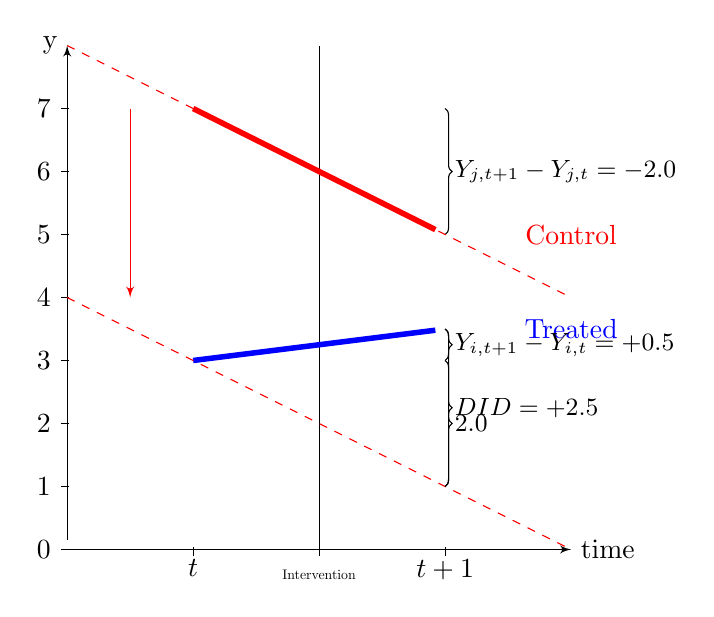
\begin{tikzpicture}[>=latex', scale=0.8]
        \draw[->] (0,0) node (origin) {}  -- (8,0) node[right] (xaxis) {time};
        \draw[->] (origin) -- (0,8) node[left] (yaxis) {y};
        % x ticks
        \foreach \x in {2,4,6}
        	\draw (\x,1pt) -- (\x,-3pt) node[anchor=north] {};
        \draw (2,0) node[below] (before) {$t$};
        \draw (6,0) node[below] (after) {$t+1$};
        \draw (4,-0.25) node[below, scale=0.5] (IV) {Intervention};
        % y ticks
        \foreach \y in {0,...,7}
             \draw (1pt,\y) -- (-3pt,\y) node[anchor=east] {$\y$};
        % intervention
        \draw (4,0) -- (4,8);

        % line
        \draw<2-> (6,3.5) node (tr) {};
        \draw<3-> (6,5) node (ctrl) {};
        \draw<2-3>[blue] (8,3.5) node (trlab) {Treated};
        \draw<3-3>[red] (8,5) node (ctrllab) {Control};        
        \draw<2->[blue, line width=2pt] (2,3) -- (tr);
        \draw<3->[red, line width=2pt] (2,7) -- (ctrl);
        
        % diffs
        \draw<4-6>[right,decorate,decoration={brace,mirror}] 
        	(6,3) -- (6,3.5) node[right, pos=0.5] (idiff) {\small $Y_{i,t+1} - Y_{i,t} = +0.5$};
        \draw<4-6>[right,decorate,decoration={brace}] 
            (6,7) -- (6,5) node[right, pos=0.5] (jdiff) {\small $Y_{j,t+1} - Y_{j,t} = -2.0$};
        
        % trends
        \draw<5-6>[red,->] (1,7) -- (1,4);
        \draw<5->[red, dashed] (0,8) -- (8,4);
        \draw<5->[red, dashed] (0,4) -- (8,0);
        \draw<6>[right,decorate,decoration={brace}] 
            (6,3) -- (6,1) node[right, pos=0.5] (idiff2) {\small $2.0$};
        \draw<7>[right,decorate,decoration={brace}] 
            (6,3.5) -- (6,1) node[right, pos=0.5] (idiff2) {\small $DID = +2.5$};
                        
        
    \end{tikzpicture}
    \end{center}
}

\frame{
	\frametitle{Lassen and Serritzlew}
	\begin{enumerate}\itemsep2em
	\item What is their research question?
	\item How do they analyze the data?
	\item What do they find and conclude?
	\end{enumerate}
}


\frame{
	\frametitle{Causal Inference Over-Time}
	\begin{itemize}\itemsep1em
		\item In experiments, matching, cross-sectional regression, and RDD, we make causal inferences based on \textbf{between-unit} comparisons at the \textit{same} time
		\item In ITS, DID, and panel analysis (next week), we make causal inferences (also) based on \textbf{within-unit} comparisons at \textit{different} times
		\item This can be really helpful, but also raises new concerns
	\end{itemize}
}



\appendix
\frame{}

\end{document}
